\chapter{Universal Clues in the Ballot Box}
\label{chap4}

Building on the empirical foundation established in Chapter 3, we now embark on a focused search for universal patterns in electoral competition. While elections vary dramatically across democracies in their rules, contexts, and scales, we aim to uncover whether fundamental statistical signatures exist that transcend these differences. This chapter presents a systematic analysis of electoral competition metrics, ultimately revealing a remarkable universality that emerges when examining the appropriate normalized measure of electoral margins.

\section{The Quest for Electoral Universality: From Previous Attempts to New Approaches}

In Chapter 3, we laid the groundwork with extensive electoral data from 34 countries across six continents. With this robust empirical foundation in place, we now turn to the central question: Do universal statistical patterns emerge in democratic competition across vastly different electoral systems?

\subsection{Historical Approaches to Electoral Universality: Prior Research and Limitations}
From a statistical physics perspective, elections represent classic complex systems where simple, universal macroscopic patterns might emerge from numerous microscopic interactions. Just as various physical systems composed of different constituent particles can exhibit the same phase transitions or scaling laws, electoral systems with different rules and contexts might share fundamental statistical signatures when properly analyzed.

Previous research has yielded partial insights but no truly robust universal electoral patterns. Various studies have examined vote share distributions and turnout patterns within specific countries \cite{CosAlmAnd1999, ForCas2007, BorBou2010} or across nations with similar electoral protocols \cite{ForCas2007, ChaMitFor2013}. Yet systematic deviations in these distributions have been repeatedly documented \cite{ChaMitFor2013, Kon2017, Kon2019, CalCroAnt2015, BorRayBou2012}, attributed to variations in electoral district size and other contextual factors.

\subsection{Exploring Universality in the Electoral Competition}

In this chapter, we undertake a systematic search for universal patterns in electoral data. We first focus on two key variables, the margin of victory and voter turnout. While the former captures the essence of democratic competition across different electoral systems, the latter sets the scale of the election. With extensive election data \cite{clea,india_data,canada_data, DVN/VOQCHQ_2018} from 34 countries (from 6 continents) spanning multiple decades and electorate scales, we analyze distributions of these variables, gradually uncovering a remarkable universal distribution. Finally, we develop a minimal statistical model that explains this universal pattern, offering insights into the fundamental nature of democratic competition.

\section{The Electoral Process: A Template}

A template of a basic electoral process is as follows. At each electoral unit, candidates compete against each other to win the votes of the electorate, who can cast their vote in favor of only one of the candidates. The candidate securing the largest number of polled votes is declared the winner. This represents the core process in many electoral systems. It is the standard first-past-the-post system followed in many countries, e.g., India, the UK, and the USA. In an instant-run-off system (such as in Australia) or two-round run-offs (such as in France), the final run-off round boils down to this template. Typically, national or regional elections following this template consist of many electoral units made up of polling booths, precincts, constituencies, or counties. These units set a size scale in terms of the number of electorates -- polling booth represents the smallest scale, while a constituency (subsuming many polling booths) represents the largest scale. For our analysis, an ``election'' could be either a national, regional, or even a city-level electoral process encompassing $N$ electoral units, and each unit could be a polling booth, county, or constituency.


In any such election, an informative indicator of the degree of competition and the extent of consensus is the margin of victory. A vanishing margin of victory signifies tight competition and a divided electorate, whereas large margins of victory indicate a decisive mandate and overwhelming consensus in favor of one candidate. Let $c_i, i=1, 2, \dots N$, denote the number of candidates contesting an election in the $i$-th electoral unit. The winning and runner-up candidates receive, respectively, $V_{i, w}$ and $V_{i, r}$ votes such that $V_{i, w} > V_{i, r}$. The margin is given by $M_i=V_{i, w}-V_{i, r}$. If $n_i > 0$ is the size of the electorate, {\it i.e.}, number of registered voters in $i$-th unit, then $0 \le M_i \le n_i$. However, in practice, only a fraction of the electorate participates in voting. In such cases, the number of voters who show up to cast their vote is termed as the turnout $T_i$, such that $0 \le T_i \le n_i$, and consequently, the margin is further restricted by $0 \le M_i \le T_i$.


\begin{figure}[h!]
    \centering
    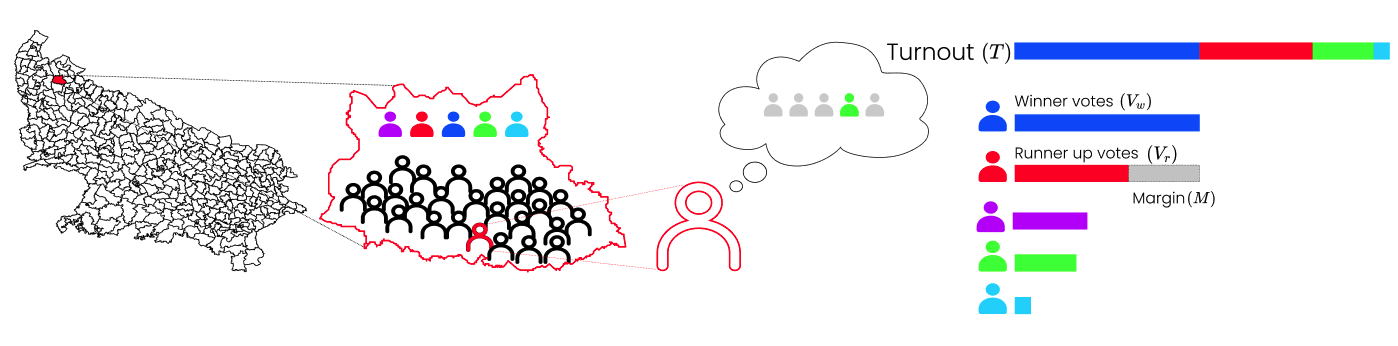
\includegraphics[width=\textwidth]{chapters/chapter4/election_template.png}
    \caption{Basic template of an election. The map highlights a single electoral unit, within a larger region. In this unit, multiple candidates (colored icons) compete for votes cast by the electorate (black icons). A representative voter casts a ballot for one candidate. The distribution of votes is summarized by key quantities on the right. The \emph{turnout} $T$ (top bar) denotes the number of participating voters and sets the scale of the contest. Among these, the candidate securing the \emph{most votes} ($V_w$, blue) is declared the winner, while the one with the \emph{second-highest votes} ($V_r$, red) is the runner-up. The \emph{margin of victory} $M = V_w - V_r$ (gray) quantifies the degree of competition -- smaller margins reflect tight races, while larger margins indicate strong consensus. This template abstracts the first-past-the-post electoral mechanism used in countries like India, the UK, and the USA, and serves as the basis for analyzing competitiveness and engagement across electoral units.}
    \label{fig:election_template}
\end{figure}


\subsection{The Dance of Turnout and Margin}

To fix our ideas, we might focus on the elections in one country, e.g., the general elections in India. Then, the object of interest would be $M_i$ and $T_i$ ($i=1,2, \dots N$). To be statistically robust, the data is consolidated from many elections spread over several decades (For India, $18$ elections from 1951 to 2019). This leads to the associated empirical distributions $Q_M(M)$ and $g(T)$, respectively, for margin and turnout. Figure \ref{fig:turnout_margin}(a) displays the distribution of raw turnout $g(T)$ at the constituency level for national elections in six countries, namely, India, USA, South Korea, Canada, Japan, and Germany. Striking dissimilarities in $g(T)$ are visible in the shape and support of distribution for countries. For Germany, $g(T)$ has a unimodal character, while that for Canada and the USA display multiple peaks. 


\begin{figure}[H]
    \centering
    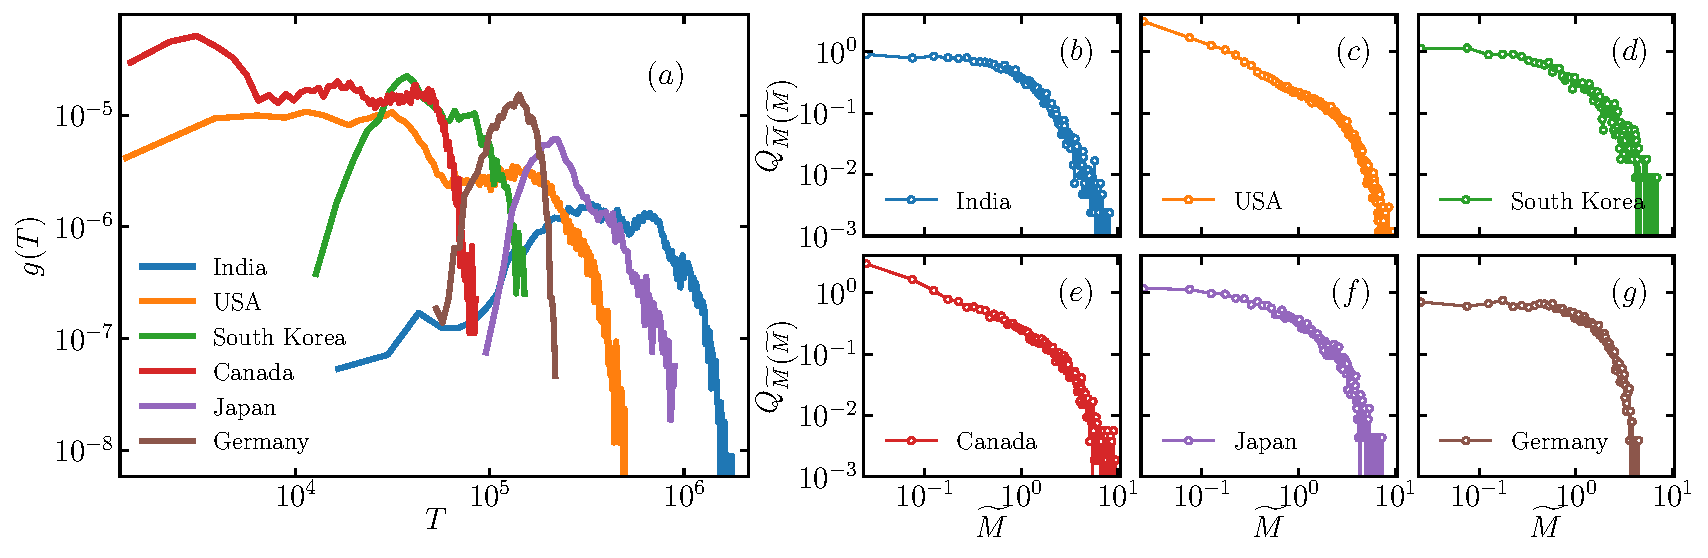
\includegraphics[width=\textwidth]{chapters/chapter4/turnout_margin_empirical_distribution_pc.pdf}
    \caption{(a) Turnout distribution $g(T)$ obtained from election data for different countries. Note the differences in shapes and ranges for $g(T)$. (b-g) Scaled margin distribution $Q_{\widetilde{M}}\left(\widetilde{M}\right)$ obtained from election data (open circles with solid lines) for India, USA, South Korea, Canada, Japan, and Germany. Despite their distinct electoral systems and political cultures, these distributions show broad similarities but also notable differences in their decay patterns.}
    \label{fig:turnout_margin}
\end{figure}

Further we scale the margin distribution with the sample mean $\langle M \rangle$, hoping the find a universal pattern. However, as displayed in Fig.~\ref{fig:turnout_margin}(b-g), the distributions of scaled margin $\widetilde{M} = M/\langle M \rangle$ (computed from the consolidated margin data for each country) demonstrate certain noticeable differences. In particular, $Q_{\widetilde{M}}\left(\widetilde{M}\right)$ for German elections in Fig.~\ref{fig:turnout_margin}(g) has a sharp cutoff, but for India and Japan in Fig.~\ref{fig:turnout_margin}(b, f) the distribution has a slower decay. 

Next, we investigate how the electoral scale affects the distributions of our key variables, an essential consideration for any claim of universality. In large countries, depending on the size of the electoral unit, the typical turnout can differ by several orders of magnitude. For example, in India, polling booths have a typical electoral size $\sim 10^3$, whereas, at the parliamentary constituency level, it is about $10^6$. Further, the shapes of $g(T)$ are also vastly different at different scales. Figure \ref{fig:scale_independence}$(a)$ captures the striking differences in range and shape of $g(T)$ for India, the US, and Canada at two different scales. The dashed lines represent smaller scales (polling booths for India and Canada, counties for the USA), while solid lines represent larger scales (constituencies for India and Canada, congressional districts for the USA). The dashed lines represent smaller scales (polling booths for India and Canada, counties for the USA), while solid lines represent larger scales (constituencies for India and Canada, congressional districts for the USA).

\begin{figure}[H]
    \centering
    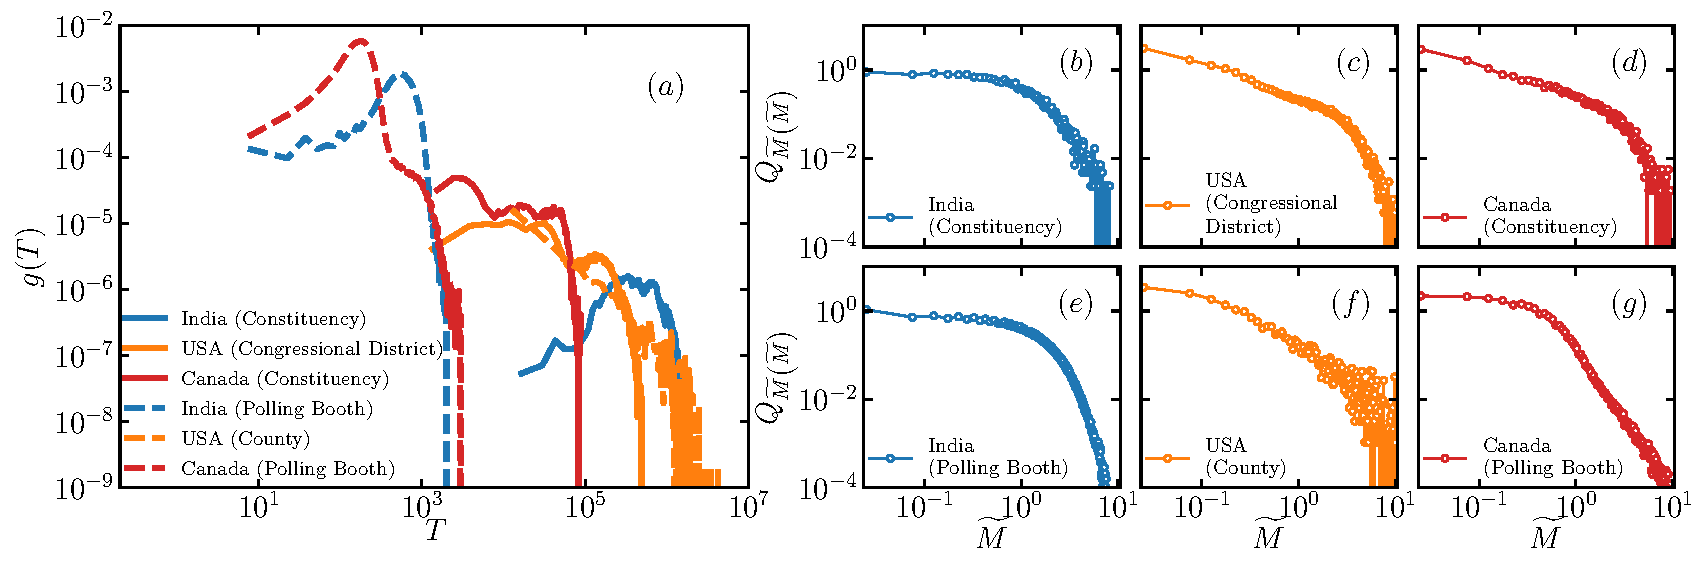
\includegraphics[width=\textwidth]{chapters/chapter4/turnout_margin_empirical_distribution_diff_scale.pdf}
    \caption{The turnout distribution $g(T)$ and scaled margin distribution $Q_{\widetilde{M}}\left(\widetilde{M}\right)$ for India (blue), the USA (orange), and Canada (red), at two widely different scales, {\it i.e.}, size of electoral units. (a) $g(T)$ at two different scales for each country. The dashed line is for smaller scales (polling booth for India and Canada, County for the USA), while the solid line represents a larger scale (constituency for India and Canada, congressional district for the USA). (b-g) $Q_{\widetilde{M}}\left(\widetilde{M}\right)$ from election data (open circles). Despite the differences in scale and shape of $g(T)$, the empirical $Q_{\widetilde{M}}\left(\widetilde{M}\right)$ shows certain consistent patterns, though scale effects are still evident.}
    \label{fig:scale_independence}
\end{figure}

The corresponding scaled margin distributions $Q_{\widetilde{M}}\left(\widetilde{M}\right)$ are shown in Figure \ref{fig:scale_independence}(b-g). Figure \ref{fig:scale_independence}$(b, c, d)$ shows the empirical distribution of scaled margins (in national elections) at the constituency-level scale, and Figure \ref{fig:scale_independence}$(e, f, g)$ shows the same at the scale of polling booths (county for USA). For each country, the distributions at different scales show certain similarities but also notable differences. For instance, in the USA, the county-level distribution (Figure \ref{fig:scale_independence}(f)) displays a heavier tail compared to the congressional district level (Figure \ref{fig:scale_independence}(c)), reflecting the influence of the underlying turnout distribution. Similar scale-dependent effects are visible in the data from India and Canada.

These variability in the scaled margin distribution, suggests that $Q_{\widetilde{M}}\left(\widetilde{M}\right)$ still carries the imprint of the underlying turnout distribution and is affected by the scale of electoral units. 

\subsection{The Need for a Scale-Independent Measure}

The variations in distributions observed across countries and scales clearly demonstrate that neither raw turnout, nor simple scaled margin can reveal universal patterns in electoral competition. The influence of electoral scale and country-specific factors persists in these measures. This suggests we need a more fundamental approach -— one that effectively normalizes out the scale effects while capturing the essential competitive dynamics common to all democratic elections. Such a measure would need to account for both the margin and the contextual scale of each electoral contest.

\section{The Specific Margin: A Scale-Invariant Approach}

Given the observed dependencies between margins and turnouts, and the constraint that $M \leq T$, we consider a new measure: the specific margin $\mu = M/T$. This ratio represents the margin normalized by the turnout at each electoral unit, producing a measure of electoral competitiveness that is independent of the size of the electorate. The specific margin $\mu$ ranges from 0 to 1, where values close to 0 indicate extremely competitive elections (nearly tied results), and values approaching 1 represent complete consensus (where nearly all voters chose the same candidate). By normalizing the margin by the local turnout, we effectively remove the scale dependency that affected our earlier analysis.


\subsection{Universal Distribution of Scaled Specific Margin}

The true breakthrough comes when we examine the scaled specific margin $\widetilde{\mu} = \mu/\langle\mu\rangle$, where $\langle\mu\rangle$ is the average specific margin for each country. Figure \ref{fig:universality_empirical} shows the distribution $Q_{\widetilde{\mu}}\left(\widetilde{\mu}\right)$ of this scaled specific margin computed from electoral data across 32 countries.

\begin{figure}[H]
    \centering
    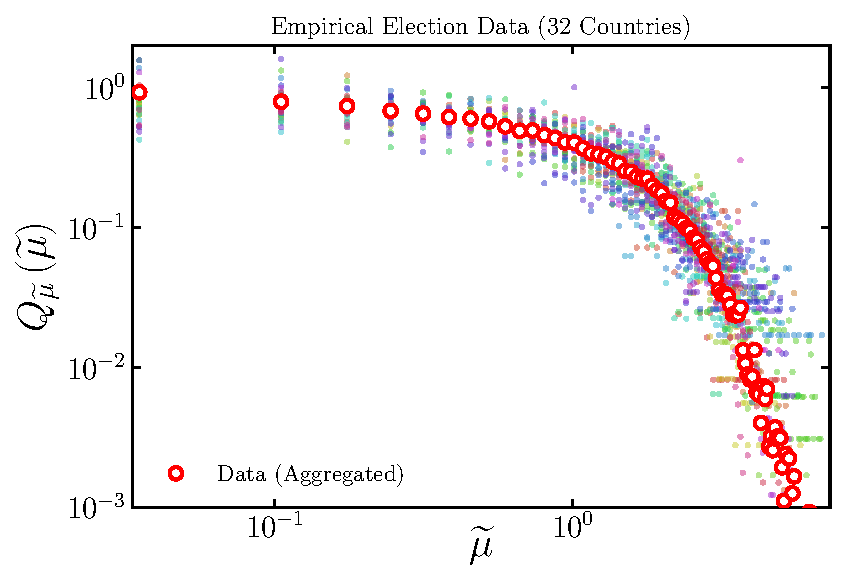
\includegraphics[width=\textwidth]{chapters/chapter4/universality_empirical.pdf}
    \caption{The empirical distribution of $\widetilde{\mu} = \mu/\langle \mu \rangle$ from election data of 32 countrie. Each color indicates a specific country for which the empirical election data is consolidated over several elections. The average of these empirical distributions is shown as red open circles.}
    \label{fig:universality_empirical}
\end{figure}

Remarkably, Figure \ref{fig:universality_empirical} reveals that the scaled specific margin distributions $Q_{\widetilde{\mu}}\left(\widetilde{\mu}\right)$, follows a universal trend across all 32 countries, despite vast differences in their electoral systems, cultural contexts, and historical backgrounds. Each colored point in the figure represents a specific country's data, and while there are small fluctuations around the aggregated distribution (attributable to finite-size effects), the overall pattern is strikingly consistent. 

This represents a remarkable finding: despite the immense complexity and diversity of electoral systems worldwide, the scaled specific margin follows a universal distribution, suggesting that the fundamental process of electoral competition—when appropriately normalized—follows the same statistical pattern regardless of where or how the election takes place.

\section{Theoretical Challenges in Explaining Statistical Universality}

While the empirical universality we've discovered is compelling, it raises a fundamental question: Why does this universal pattern emerge across such diverse electoral systems? What underlying mechanism could generate such consistent statistical behavior despite the vast differences in political contexts, voter behaviors, and electoral rules?

\subsection{A Glimpse of the Mechanism: The Random Voting Model}

The consistency of the pattern suggests that there might be a simple but powerful statistical principle at work—something fundamental to the process of competitive selection itself, rather than specific to electoral politics. The universality we've discovered hints that once turnout is ``normalized out" through the specific margin, what remains is a fundamental statistical process common to all competitive elections, suggesting that a minimal model focused on the core statistical features of electoral competition might be sufficient to explain the observed universality.

With this insight we propose a simple stochastic model, called the Random Voting Model (RVM). In this model, each voter in a constituency selects one of the candidates according to \emph{some} probability $p_j$ for $j=1,2,3$. While in the next chapter we address the precise choice of these probabilities as well as the detailed analysis of the model, for now, we focus on their statistical consequences. We solve the model in the limit of large turnout $(T \gg 1)$, meaning when the number of voters is sufficiently large. In this limit, the votes received by the $j$-th candidate can be approximated as $v_j \approx p_jT$ (the probability of voting for that candidate multiplied by the turnout), and the margin of victory as $M \approx \left(p_{(3)} - p_{(2)}\right) T$, where $p_{(k)}$ denotes the $k$-th order statistic \cite{BarBalNag2008} of the probabilities assigned to the candidates -— in simpler terms, $p_{(3)}$ is the probability of the winner and $p_{(2)}$ is the probability of the runner-up. Evidently, in this limit, the specific margin $\mu \approx p_{(3)} - p_{(2)}$ becomes the difference between these probabilities and its distribution has no explicit dependence on turnout $T$. With this insight, we obtain the distribution of specific margins as:

\begin{equation}
    Q_{\mu}(\mu) = \frac{(1 - \mu)(5 + 7\mu)}{(1 + \mu)^2(1 + 2\mu)^2}.
\end{equation}

Thus, the distribution $Q_{\widetilde{\mu}}\left(\widetilde{\mu}\right)$ of the scaled specific margin $\widetilde{\mu} = \mu/\langle\mu\rangle$ is:

\begin{equation}
    Q_{\widetilde{\mu}}\left(\widetilde{\mu}\right) = \langle\mu\rangle Q_{\mu}\left(\widetilde{\mu}\langle\mu\rangle\right),
    \label{eq:Fscale}
\end{equation}

with $\langle\mu\rangle = \frac{1}{2} + \ln\left(\frac{9\sqrt[4]{3}}{16}\right)$ and the distribution is independent of the underlying turnout distribution $g(T)$.

\begin{figure}[H]
    \centering
    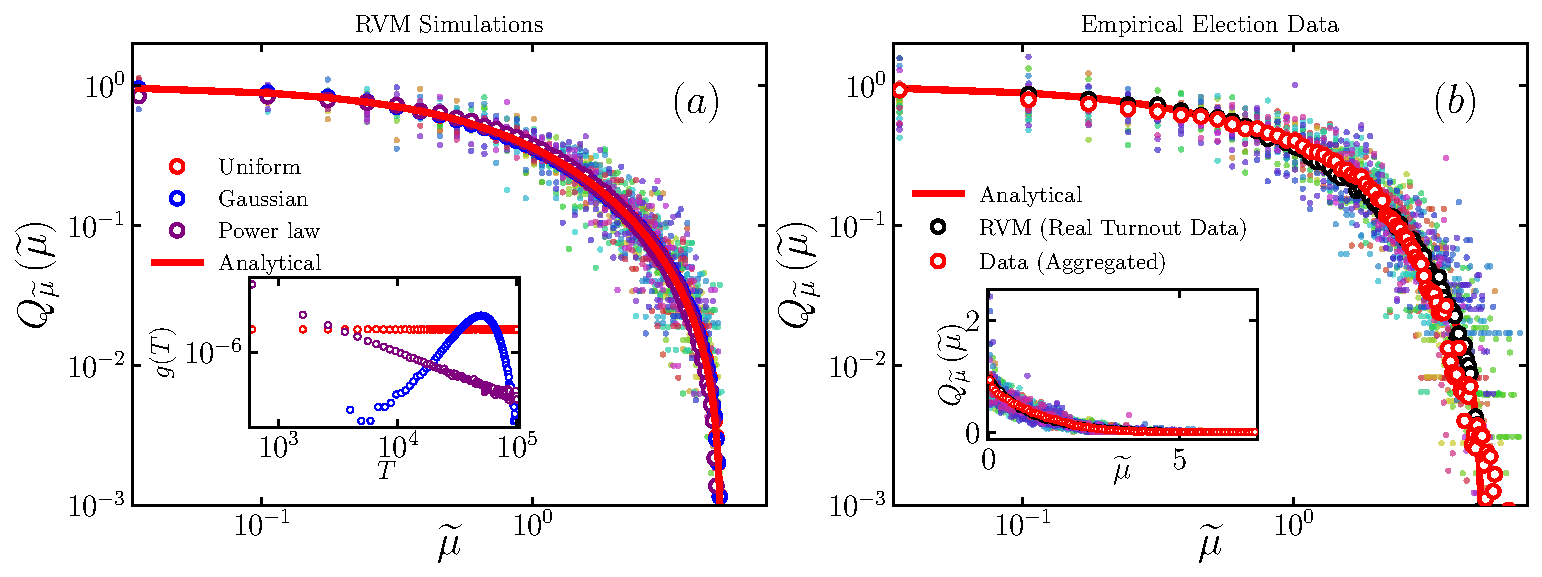
\includegraphics[width=\textwidth]{chapters/chapter4/universality_simulation_empirical_analytical.pdf}
    \caption{(a) $Q_{\widetilde{\mu}}\left(\widetilde{\mu}\right)$ predicted by RVM for three different turnout distributions $g(T)$ (see inset). The open circles are obtained from RVM simulations with $N = 10^6$, while the solid colored circles are generated from RVM simulation with $N$ identical to empirical election data. The red line corresponds to $Q_{\widetilde{\mu}}\left(\widetilde{\mu}\right)$ in Eq. \ref{eq:Fscale}. (b) The empirical distribution of $\widetilde{\mu} = \mu/\langle \mu \rangle$ from election data of 32 countries (excluding Ethiopia and Belarus). Each color indicates a specific country for which the empirical election data is consolidated over several elections. The average of these empirical distributions (red open circles) closely follows the analytical curve (red line) and the averaged RVM predictions for each country (black open circles). The inset depicts the distributions on a linear scale.}
    \label{fig:universality}
\end{figure}


In figure \ref{fig:universality}(a) we demonstrate that $Q_{\widetilde{\mu}}\left(\widetilde{\mu}\right)$, computed from RVM simulations with vastly different turnout distributions $g(T)$, does not depend on the detailed structure of $g(T)$ and is in agreement with the analytical prediction in Eq. \ref{eq:Fscale}. The RVM simulations are performed with $10^6$ electoral units using $g(T)$ corresponding to power law, Gaussian, and uniform distributions (inset of Fig.~\ref{fig:universality}(a)). The simulated distributions (open circles in Fig.~\ref{fig:universality}(a)), for the three cases of $g(T)$, collapse on the analytical prediction $Q_{\widetilde{\mu}}\left(\widetilde{\mu}\right)$ (red line). 

We further examine if prediction in Eq. \ref{eq:Fscale} holds good for the empirical election data. Indeed, as observed in Fig.~\ref{fig:universality}(b), the RVM prediction (black open circles) is in excellent agreement with the averaged distributions (open red circles) obtained from all the $32$ countries. The averaged empirical distribution is also consistent with the analytical universal curve $Q_{\widetilde{\mu}}\left(\widetilde{\mu}\right)$ (red line). Further, the empirical distribution for each of the $32$ countries (denoted by the solid-colored circles) closely follows the trend of $Q_{\widetilde{\mu}}\left(\widetilde{\mu}\right)$, albeit with some fluctuations induced by the finite size of data. Similar fluctuations are evident in RVM simulations as well, seen as solid circles in Fig.~\ref{fig:universality}(a), when the number of electoral units $N$ is taken from the empirical election data (rather than fixed at $10^6$). Empirical distributions shown in the inset of Fig.~\ref{fig:universality}(b) demonstrate that at large $x$, the absolute fluctuations decrease. 

Thus, the universality in Fig.~\ref{fig:universality} suggests that irrespective of the finer details of election processes, the mechanism underlying the core component of any competitive election -- choosing one candidate from many contenders -- leads to a universal distribution for the scaled specific margin $\widetilde{\mu}=\mu/\langle \mu \rangle$. This remarkable agreement between our simple Random Voting Model and empirical data from diverse democracies suggests that we have identified a fundamental statistical signature of democratic competition that transcends specific electoral systems and cultural contexts. 

\section{Conclusion: Universality as a Signature of Democratic Competition}

In this chapter, using extensive election data from 32 countries spanning multiple decades and electorate scales, we have demonstrated a remarkable statistical universality in democratic electoral competition. While raw turnout distributions vary dramatically across countries and scales, and scaled margin distributions retain country-specific features, the scaled specific margin follows a universal distribution across 32 diverse democracies.

This universality transcends the particularities of individual countries, electoral systems, and scales, revealing what appears to be a fundamental statistical signature intrinsic to competitive democratic processes. Like other universalities discovered in complex systems, this pattern emerges not despite but because of the underlying complexity, as coherent patterns can arise from the aggregation of many individual decisions. We further argue that this universality is a stylized fact of elections and any successful election model should be able to reproduce it.

The elegance of this finding lies in its simplicity: once we properly normalize the margin by the local turnout and scale by the country-specific mean, the resulting distribution follows a consistent pattern regardless of cultural, historical, or institutional factors. It suggests that beneath the surface complexity of electoral politics lies a simpler statistical regularity, which is a signature of democratic competition, which we capture with our proposed Random Voting Model.

Building on the success of the RVM in explaining this universal pattern, the next chapter will provide a comprehensive analysis of the model from first principles. We will derive its mathematical foundations, demonstrate how it connects turnout distributions to margin distributions across different electoral contexts, and explore how this elegantly simple model can explain multiple empirical findings.